\documentclass[sigconf]{acmart}
% Local preview support; replace with the organizer's preamble when available.
\newif\ifguideStyle
\newcommand{\guide}[1]{%
  \ifguideStyle
    {\color{gray!65}\itshape #1}%
  \fi
}

\guideStylefalse
\setcopyright{none}
\settopmatter{printacmref=false}
\acmConference[Technical Report]{Competition Technical Report}{November 2026}{Online}
\acmYear{2026}
\acmDOI{}
\acmISBN{}
\setlength{\emergencystretch}{1em}
\setcounter{dbltopnumber}{3}
\renewcommand{\dbltopfraction}{0.95}
\renewcommand{\textfraction}{0.05}

\begin{document}
\title{From Pixels to Instances: A Visual Study of Solar Filament Segmentation}
\subtitle{A Solution to the Solar Filament Segmentation Challenge 2026}
\author{Gregory Kojadinovich II}
\affiliation{%
  \institution{Europa Waters LLC}
  \city{South Lake Tahoe, CA}
  \country{USA}
}
\email{gregkoja3343@icloud.com}

\begin{abstract}
We present a visual account of four computer-vision experiments for
segmenting solar filaments in grayscale GONG H-$\alpha$ images. Public
Kaggle Panoptic Quality (PQ) progressed from 0.29 for a ResNet18 U-Net
baseline, to 0.32 after higher-resolution, contrast-enhanced fine-tuning,
and to 0.35 with YOLO11s instance proposals, crop refinement, and repaired
disjoint-mask export. A fourth experiment, V5, trains five independent
YOLO/ResNet34-U-Net pairs and combines their predictions, reaching PQ 0.36.
Original diagrams, training curves, and prediction overlays explain
the changes and evidence limits. The 0.07 absolute gain is a pipeline
progression, not an isolated causal effect. This visual V2 draft retains
the first paper separately.
\end{abstract}

\begin{teaserfigure}
\centering
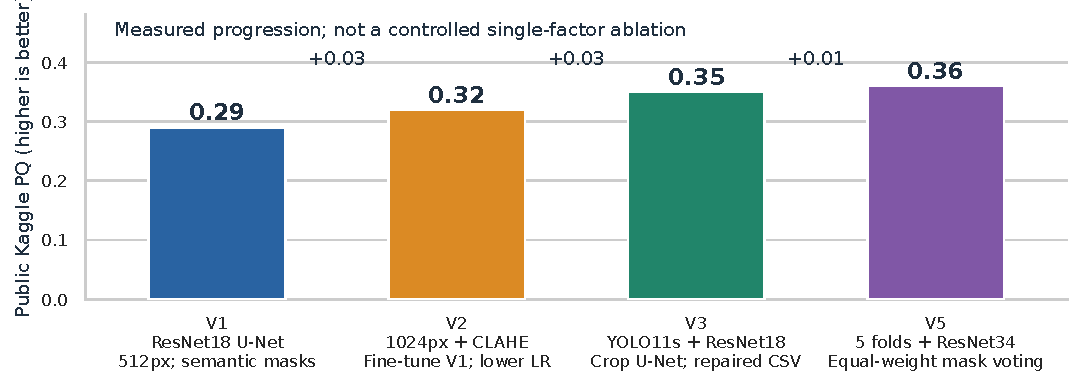
\includegraphics[width=\textwidth]{figures-v2/score_progression.pdf}
\caption{The measured competition progression. V2 denotes focused fine-tuning,
not the separate grouped V2 research notebook. V3 is the accepted, repaired
submission. V5 is the accepted five-fold ensemble (0.36). Labels identify
headline changes associated with each experiment; they do not prove which
change caused a gain. PQ measures instance segmentation, not pixel accuracy.}
\label{fig:scores}
\end{teaserfigure}
\maketitle

\section{Question and Research Context}
How can an applied segmentation pipeline better preserve and separate thin
solar filaments while producing valid competition instances? The
MAGFiLO-based challenge~\cite{filament-segmentation-2026,ahmadzadeh2024dataset}
provides grayscale intensity images and annotator-specific masks.
They are not magnetograms; we do not infer magnetic-field values.
Gregory Kojadinovich II, developer and founder of Europa Waters LLC,
leads this engineering study.

The ESAIR poster by Singh et al.~\cite{esairposter2026} emphasizes thin
boundaries, multiscale IoU loss, grouping fragmented U-Net regions through
spine proximity/orientation, and subsequent chirality classification with
ConvNeXt. Our contribution is complementary but narrower: compare
semantic versus instance-aware prediction, diagnose mask failures, and
produce traceable, nonoverlapping instance exports. We use Dice/BCE for
U-Net training, not ESAIR's multiscale-IoU loss; we do not implement its
grouping algorithm or train a chirality classifier.

\begin{figure*}[t]
\centering
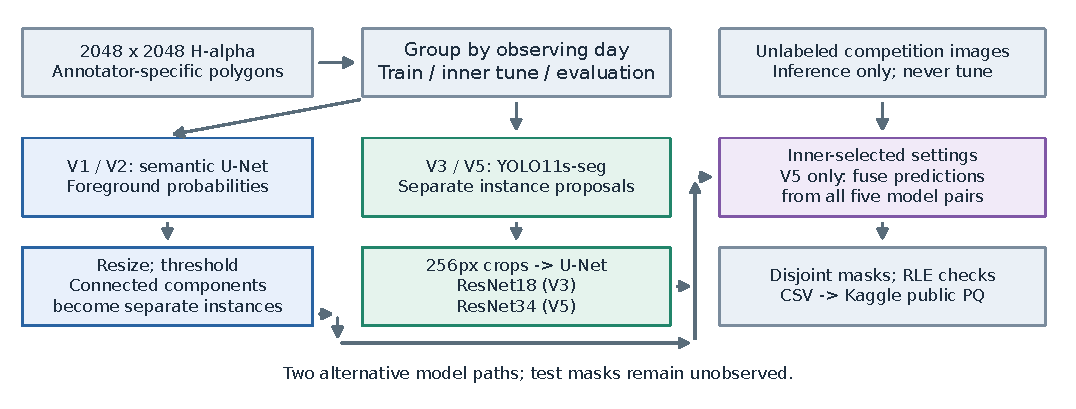
\includegraphics[width=\textwidth]{figures-v2/workflow.pdf}
\caption{Original, Visio-style pipeline diagram. V1/V2 derive instances from
a semantic foreground map; V3/V5 predict instances before local refinement.
The two colored branches are alternatives, not sequentially trained stages
of one network. Training, calibration, evaluation, and competition inference
have distinct roles.}
\label{fig:workflow}
\end{figure*}

\begin{figure*}[t]
\centering
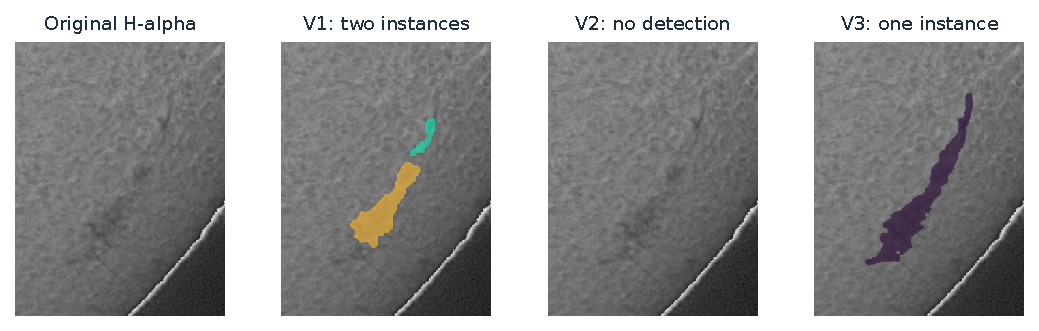
\includegraphics[width=\textwidth]{figures-v2/mask_comparison.pdf}
\caption{Actual saved predictions on one disagreement-selected test crop,
not ground truth: \texttt{20210708060030Lh.jpeg}, original
$x=[1502,1767)$, $y=[1328,1673)$. V1 splits the visible structure into
two predicted instances, V2 retains none in this crop, and V3 produces
one larger instance. Colors identify predicted objects, not correctness.
Selection targets disagreement, not a representative accuracy estimate.
This illustration cannot establish which boundary is correct.}
\label{fig:masks}
\end{figure*}

\begin{figure*}[t]
\centering
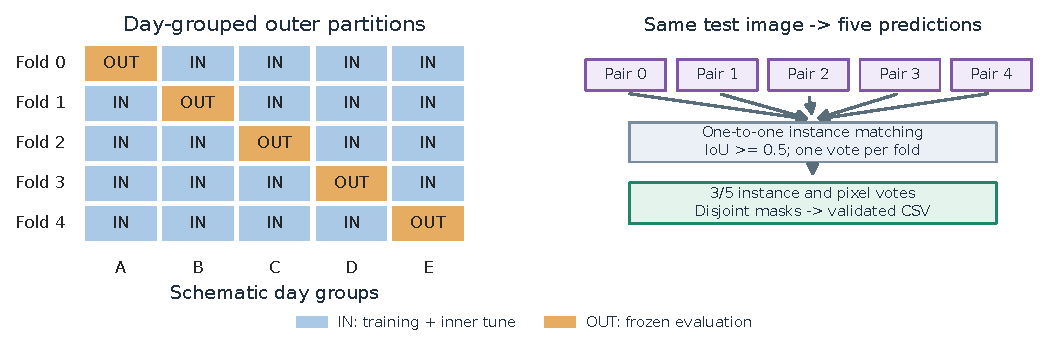
\includegraphics[width=\textwidth]{figures-v2/folds_and_fusion.pdf}
\caption{Left: schematic outer-day assignment, not equally sized actual
image bins. Each IN partition is further split into training and inner
tuning; OUT is never used for that model's selection. Right: all five
trained model pairs predict the same unlabeled test image. Instance
matching and fixed majority voting form a submission; raw instance lists
are not simply concatenated.}
\label{fig:folds}
\end{figure*}

\begin{figure*}[t]
\centering
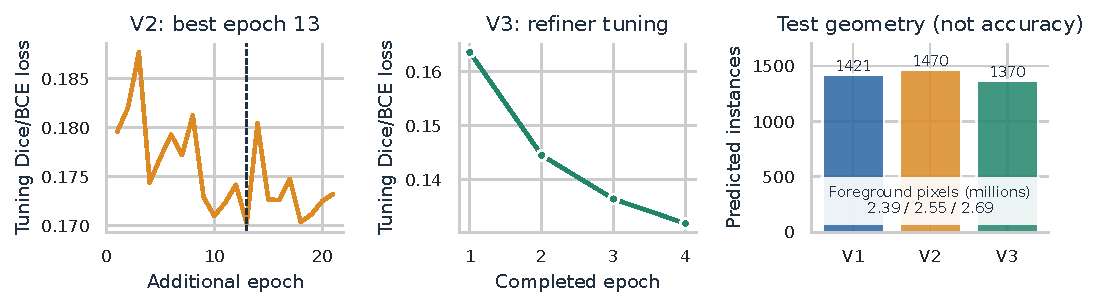
\includegraphics[width=\textwidth]{figures-v2/training_and_geometry.pdf}
\caption{Measured diagnostics, not a causal ablation. Left: focused V2
selects additional epoch 13 before early stopping at 21. Center: V3 refiner
tuning loss improves through all four completed epochs, motivating further
training without guaranteeing improved PQ. Right: across 180 test images,
V3 predicts fewer instances but more foreground than V2. All data come from
saved training/EDA artifacts. Losses across different datasets/models must
not be read as a common accuracy scale.}
\label{fig:diagnostics}
\end{figure*}

\section{Data and Evaluation: What Is Kept Separate?}
The dataset contains 707 labeled photographs, 1154 annotator image sets,
8199 instance annotations, and 180 unlabeled competition images.
Annotators may outline the same filament; polygons form one foreground class.

V1--V3 use one day-grouped split: 499 training, 103 tuning, and 105 holdout
photographs (seed 2026). All annotator targets stay with their photograph.
Tuning selects checkpoints/postprocessing; holdout labels do not.
Local metrics average annotators within photographs, then photographs.
Reused development data are not an untouched final benchmark.

PQ~\cite{pq} rewards both instance overlap and recognition:
\begin{equation}
 \mathrm{PQ}=
 \frac{\sum_{(p,g)\in TP}\mathrm{IoU}(p,g)}
 {|TP|+\tfrac12|FP|+\tfrac12|FN|}.
\end{equation}
Local matching requires IoU strictly greater than 0.5. Dice, IoU,
detector mAP, and public PQ are not interchangeable. No repeated-seed
error bars are available for the single-run public scores.

\section{Which Change Accompanied Each Score Gain?}
\subsection{V1: Establish a Semantic Baseline (0.29)}
A U-Net~\cite{unet} with an ImageNet-pretrained ResNet18
encoder~\cite{resnet} predicts one foreground probability per pixel.
Images are resized from 2048 to 512 pixels per side, normalized to
$[-1,1]$, and augmented with paired rotations/flips. AdamW uses
$3\times10^{-4}$ learning rate, batch eight, and 20 epochs. The loss is
equal-weight BCE and soft Dice. Full-resolution probabilities are
thresholded; eight-connected components become instances.
This simple representation can merge touching filaments or split
disconnected parts. Submission 58301531 achieved public PQ 0.29.

\begin{figure}[t]
\centering
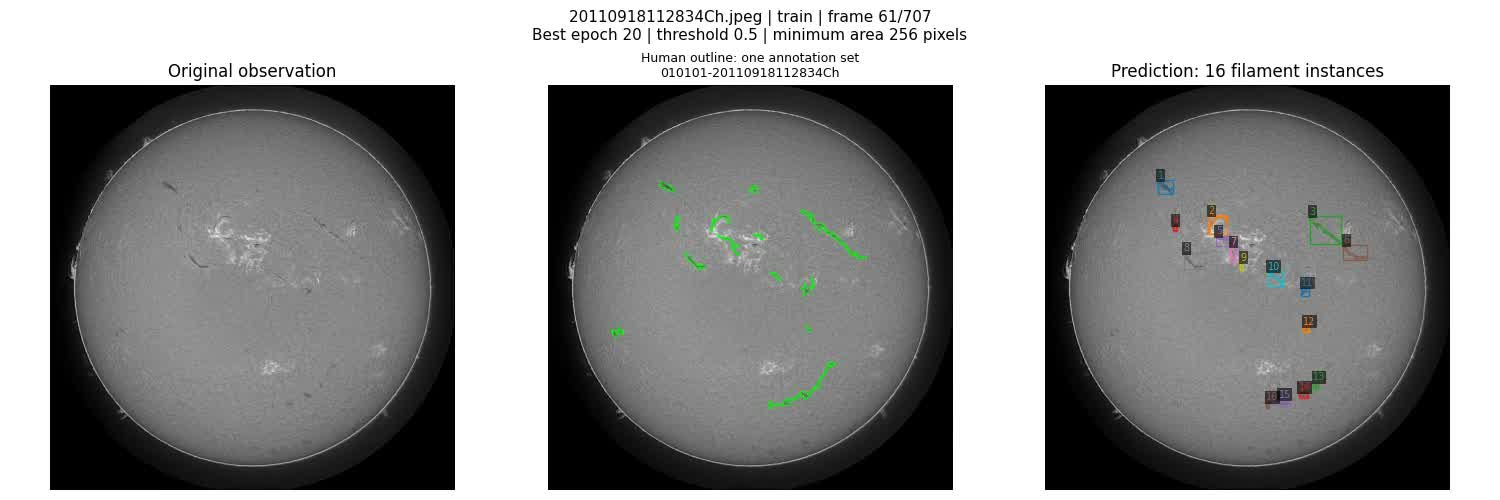
\includegraphics[width=\linewidth]{../Baseline Video/thumbnail.jpg}
\caption{Frame from the baseline review video showing the observation,
human annotation, and model overlay with component-derived boxes. The
sequence includes training images; this qualitative example is not an
independent performance estimate.}
\label{fig:baseline-review}
\end{figure}

\subsection{V2: More Detail and Local Contrast (0.32; +0.03)}
The \emph{headline change} is a higher-detail input: 1024 pixels per side
with CLAHE~\cite{opencvclahevisual} (clip limit two; $8\times8$ tile grid).
V2 fine-tunes V1's weights with a fresh AdamW optimizer,
$10^{-4}$ learning rate, batch two, plateau scheduling, and early stopping.
It completes 21 additional epochs and selects additional epoch 13.
Submission 58304132 achieves public PQ 0.32.

Finer sampling may preserve faint filaments. However, resolution, contrast,
schedule, and training continuation changed together; the +0.03 cannot be
attributed to CLAHE or resolution alone.

\subsection{V3: Learn Instances Before Refining Pixels (0.35; +0.03)}
The \emph{headline change} is instance-aware prediction:
YOLO11s-seg~\cite{ultralyticsvisual} at 1024 pixels proposes distinct objects;
an ImageNet-pretrained ResNet18 U-Net refines local crops.
For each instance, a square covering 1.8 times its largest extent
(minimum side 96 pixels, clipped to the frame) is resized to $256^2$.
The grayscale crop is replicated into three channels for the pretrained
refiner. Its output is resized to the original crop before thresholding.
Annotation-bound training crops differ from detector-bound inference crops;
refinement cannot recover missed proposals.

V3 completes 47 detector epochs and part of epoch 48 within its detector
allowance, but only four complete refiner epochs. Its initial CSV is
rejected for overlapping masks. Offline repair retains earlier masks,
removes contested pixels from later ones, and drops remnants below 20
pixels, without retraining. Accepted submission 58316663 scores 0.35.
The +0.03 reflects the complete repaired pipeline, not proof that the
refiner alone caused the gain. Pre-repair tuning PQ does not measure the
repaired predictions.

\section{V5: Five Model Pairs, One Ensemble Submission}
\subsection{What Is Actually Trained?}
V5 is the fourth principal experiment; V4 was a separate long-training
attempt with no reported competition score. V5 trains \emph{five independent}
YOLO11s-seg/ResNet34-U-Net pairs, one per day-grouped fold.
The detectors initialize from pretrained YOLO weights; each refiner
initializes its encoder from ImageNet, with a newly initialized decoder/head.
These networks are fine-tuned; pretrained does not mean frozen.
The ensemble itself has no learned parameters or separate optimizer.

Each outer fold contains about 20\% of labeled images; 10\% of remaining
days is inner tuning, yielding approximately 72/8/20 train/tune/outer
percentages. Fold training counts are 510, 510, 508, 511, and 512 physical
images. Outer partitions cover each photograph once; evaluation after inner
selection reduces selection bias~\cite{varma2006}.

\subsection{Fixed Budgets and Frozen Fusion Rules}
Per-fold ceilings are five YOLO epochs and two refiner epochs, or 25
detector and ten refiner epochs across all pairs. Detector/refiner input
sizes remain 1024/256 and batches four/16. Explicit AdamW uses
detector LR 0.002 and refiner LR 0.0003; the refiner uses cosine scheduling.
Up to eight inner images calibrate confidence, crop threshold, minimum
area, and YOLO-only versus refined output separately per fold.

The two-hour cooperative target reserves 20 minutes for export.
The remaining pre-minute-100 time is split among unfinished folds;
40\% of each fold allowance goes to YOLO, the rest to refinement.
Calibration/evaluation/export are not hard-limited. Incomplete refiner
epochs are discarded. Partial logs show five detector epochs but just
one completed refiner epoch in each of folds 0 and 1. Final execution
counts/runtime await full logs. Fold 4's missing refiner was recovered
without a deadline; this run did not meet the two-hour target.

All five models predict each test image with their inner-selected settings.
One-to-one instance matching uses IoU at least 0.5 against running cluster
representatives, in fixed fold order. Instances and pixels need three of
five votes. A 20-pixel area filter and support-then-area disjoint ownership
remove small/overlapping remnants. Zero detections are audited, not filled
with invented masks. IDs, RLE roundtrips, readback, and zero overlaps are checked.

\subsection{V5: Accepted PQ 0.36 (+0.01)}
Submission 58327117 achieved 0.36. The +0.01 over V3 measures the \emph{whole procedure},
not the isolated benefit of ResNet34 or pretraining: V3 already uses an
ImageNet-pretrained ResNet18 refiner. Split, training exposure, depth, and
fusion change together. No random-initialization or individually scored
V5-fold comparison has been measured.

Outer mean/SD describe individual held-out models, not ensemble performance:
other models have seen those images. Voting may remove false positives
or true low-agreement filaments.

\section{What the Visual Evidence Establishes}
The +0.07 absolute PQ progression (about 24.1\% relative to 0.29)
is not a seven-percentage-point increase in pixel accuracy.
V3 contains 253 disconnected masks; V1/V2's connected-component extraction
cannot produce such instances. All three omit the same three test images.
Prediction morphology alone does not establish correctness.

Priority controls are single fold versus ensemble, ResNet18 versus ResNet34,
and pretrained versus random encoders, under fixed evaluation and repeated
seeds. ESAIR's boundary loss/grouping would be separate experiments.
Pixel-error overlays diagnose boundaries; instance-IoU matching diagnoses
splits and merges. Headline changes remain plausible mechanisms, not causes.

A separate unscored V6 prepares 25/20-epoch ceilings, early stopping
without wall-clock truncation, cached crops, batched inference, and two-GPU refinement.
Neither speedup nor higher PQ has been measured.

\section{Reproducibility and Submission Status}
The repository\footnote{\href{https://github.com/Greg-Kojadinovich/solar-filament-segmentation-2026}{Public source repository on GitHub.}}
links notebooks, tests, and EDA. Submission identifiers accompany
Figure~\ref{fig:scores}'s source data. The plotting script retains input
hashes. Diagrams are original editable SVGs and vector PDFs; observation
panels remain raster. ESAIR's poster artwork is not reproduced.

Complete V5 reproduction additionally requires all five checkpoint pairs,
matching plan/calibration files, actual environment versions, completed
epoch counts, and runtime. The verified V5 CSV contains 1127 disjoint masks
across 177 images; its SHA-256 is recorded with the figure inputs.
An earlier upload selected stale V3 output and was rejected, not scored.
The organizers require a technical report and public code link through their
judging form before the stated November 15 deadline~\cite{filamentannouncements};
prediction submission alone is not report submission.
Their August announcement values PQ strictly greater than 0.35;
V5's 0.36 exceeds that stated threshold, not proof of operational readiness.

\clearpage
\section{Acknowledgment}
The organization of the Filament Segmentation Challenge 2026 is partially
supported by the U.S. National Science Foundation (NSF) under Grant No.
2209912 and 2433781, directorate for Computer and Information Science and
Engineering (CSE), and Office of Advanced Cyberinfrastructure (OAC), and
Grant No. 2511630, AST Division Of Astronomical Sciences and MPS Directorate
for Mathematical and Physical Sciences.

The Filament Segmentation Challenge 2026 is sponsored by the U.S. National
Science Foundation (NSF) National Solar Observatory (NSO).

This work utilizes GONG data obtained by the NSO Integrated Synoptic Program,
managed by the National Solar Observatory, which is operated by the
Association of Universities for Research in Astronomy (AURA), Inc. under a
cooperative agreement with the National Science Foundation and with
contribution from the National Oceanic and Atmospheric Administration.
The GONG network of instruments is hosted by the Big Bear Solar Observatory,
High Altitude Observatory, Learmonth Solar Observatory, Udaipur Solar
Observatory, Instituto de Astrofisica de Canarias, and Cerro Tololo
Interamerican Observatory.

\bibliographystyle{ACM-Reference-Format}
\bibliography{main,poster_v2}
\end{document}
